\chapter{Experimental results}
After the analysis of the training and validation data, the choice fell to the TDNN, because compared to the RNN:
\begin{itemize}
	\item has got better validation accuracy and a smaller loss value;
	\item in almost every test, showed smoother training and validation curves, and was easier to train effectively.
\end{itemize}
Follows a comparison between the networks' testing results, based on confusion matrices, accuracy and F1 score (for the theoretical concepts see section \ref{Evaluate neural networks}).

\begin{table}[ht!]
	\centering
	\begin{tabular}{c|cccccc}
		& \textbf{Backward} & \textbf{Flight} & \textbf{Forward} & \textbf{Still} & \textbf{Thrown} & \textbf{Walking} \\ \hline
		\textbf{Backward} & 19                & 0               & 0                & 1              & 0               & 0                \\
		\rowcolor[HTML]{EFEFEF} 
		\textbf{Flight}   & 1                 & 49              & 0                & 0              & 0               & 0                \\
		\textbf{Forward}  & 0                 & 0               & 20               & 0              & 0               & 0                \\
		\rowcolor[HTML]{EFEFEF} 
		\textbf{Still}    & 0                 & 0               & 0                & 50             & 0               & 0                \\
		\textbf{Thrown}   & 0                 & 0               & 1                & 0              & 46              & 3                \\
		\rowcolor[HTML]{EFEFEF} 
		\textbf{Walking}  & 0                 & 1               & 0                & 0              & 0               & 49              
	\end{tabular}
	\caption{TDNN's confusion matrix.}
\end{table}

\begin{table}[ht!]
	\centering
	\begin{tabular}{c|cccccc}
		\textbf{}         & \textbf{Backward} & \textbf{Flight} & \textbf{Forward} & \textbf{Still} & \textbf{Thrown} & \textbf{Walking} \\ \hline
		\textbf{Backward} & 19                & 0               & 0                & 0              & 1               & 0                \\
		\rowcolor[HTML]{EFEFEF} 
		\textbf{Flight}   & 0                 & 47              & 1                & 0              & 0               & 2                \\
		\textbf{Forward}  & 0                 & 1               & 18               & 0              & 0               & 1                \\
		\rowcolor[HTML]{EFEFEF} 
		\textbf{Still}    & 0                 & 0               & 0                & 50             & 0               & 0                \\
		\textbf{Thrown}   & 0                 & 0               & 0                & 0              & 50              & 0                \\
		\rowcolor[HTML]{EFEFEF} 
		\textbf{Walking}  & 0                 & 5               & 1                & 0              & 0               & 44              
	\end{tabular}
	\caption{RNN's confusion matrix.}
\end{table}

\begin{center}
	\begin{figure}[ht!]
		\makebox[\textwidth]{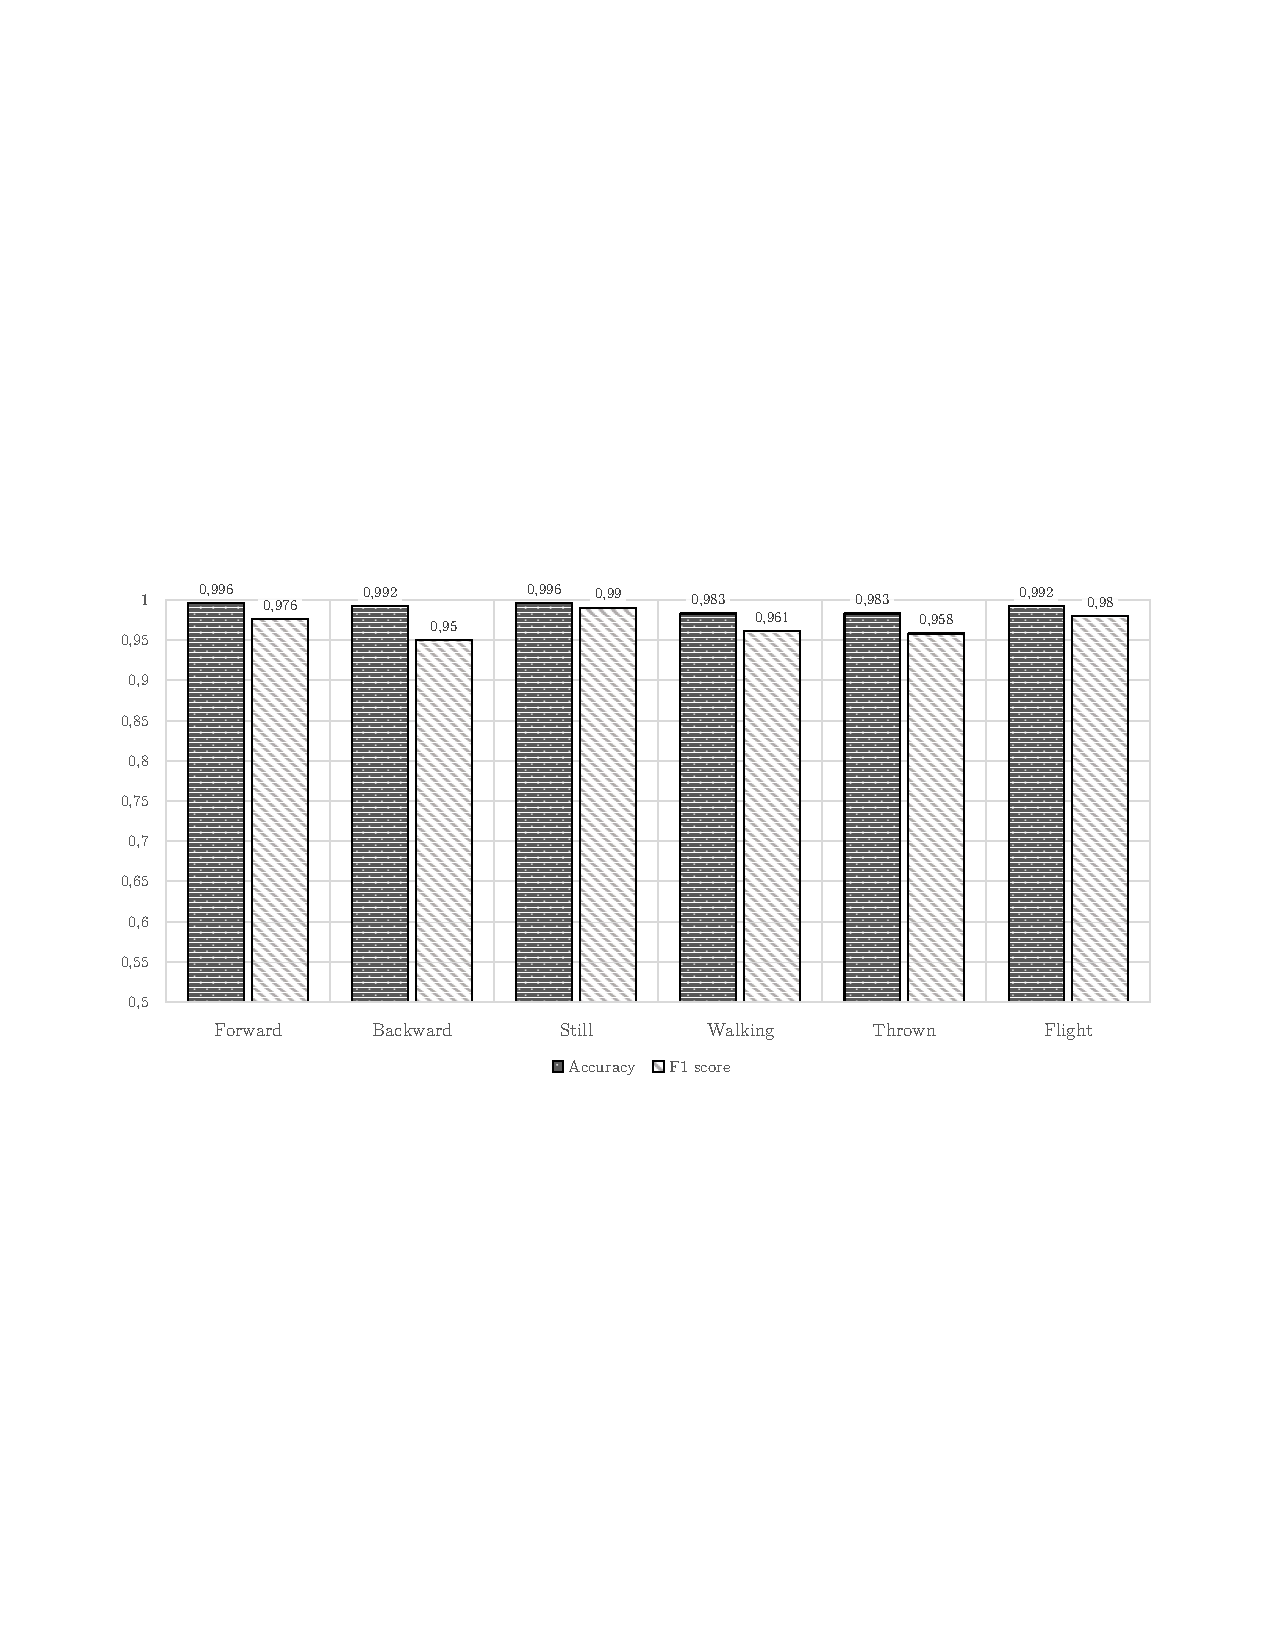
\includegraphics[width=0.8\paperwidth]{img/tdnn_results.pdf}}
		\caption{TDNN testing results.}
	\end{figure}
\end{center}

\begin{center}
	\begin{figure}[ht!]
		\makebox[\textwidth]{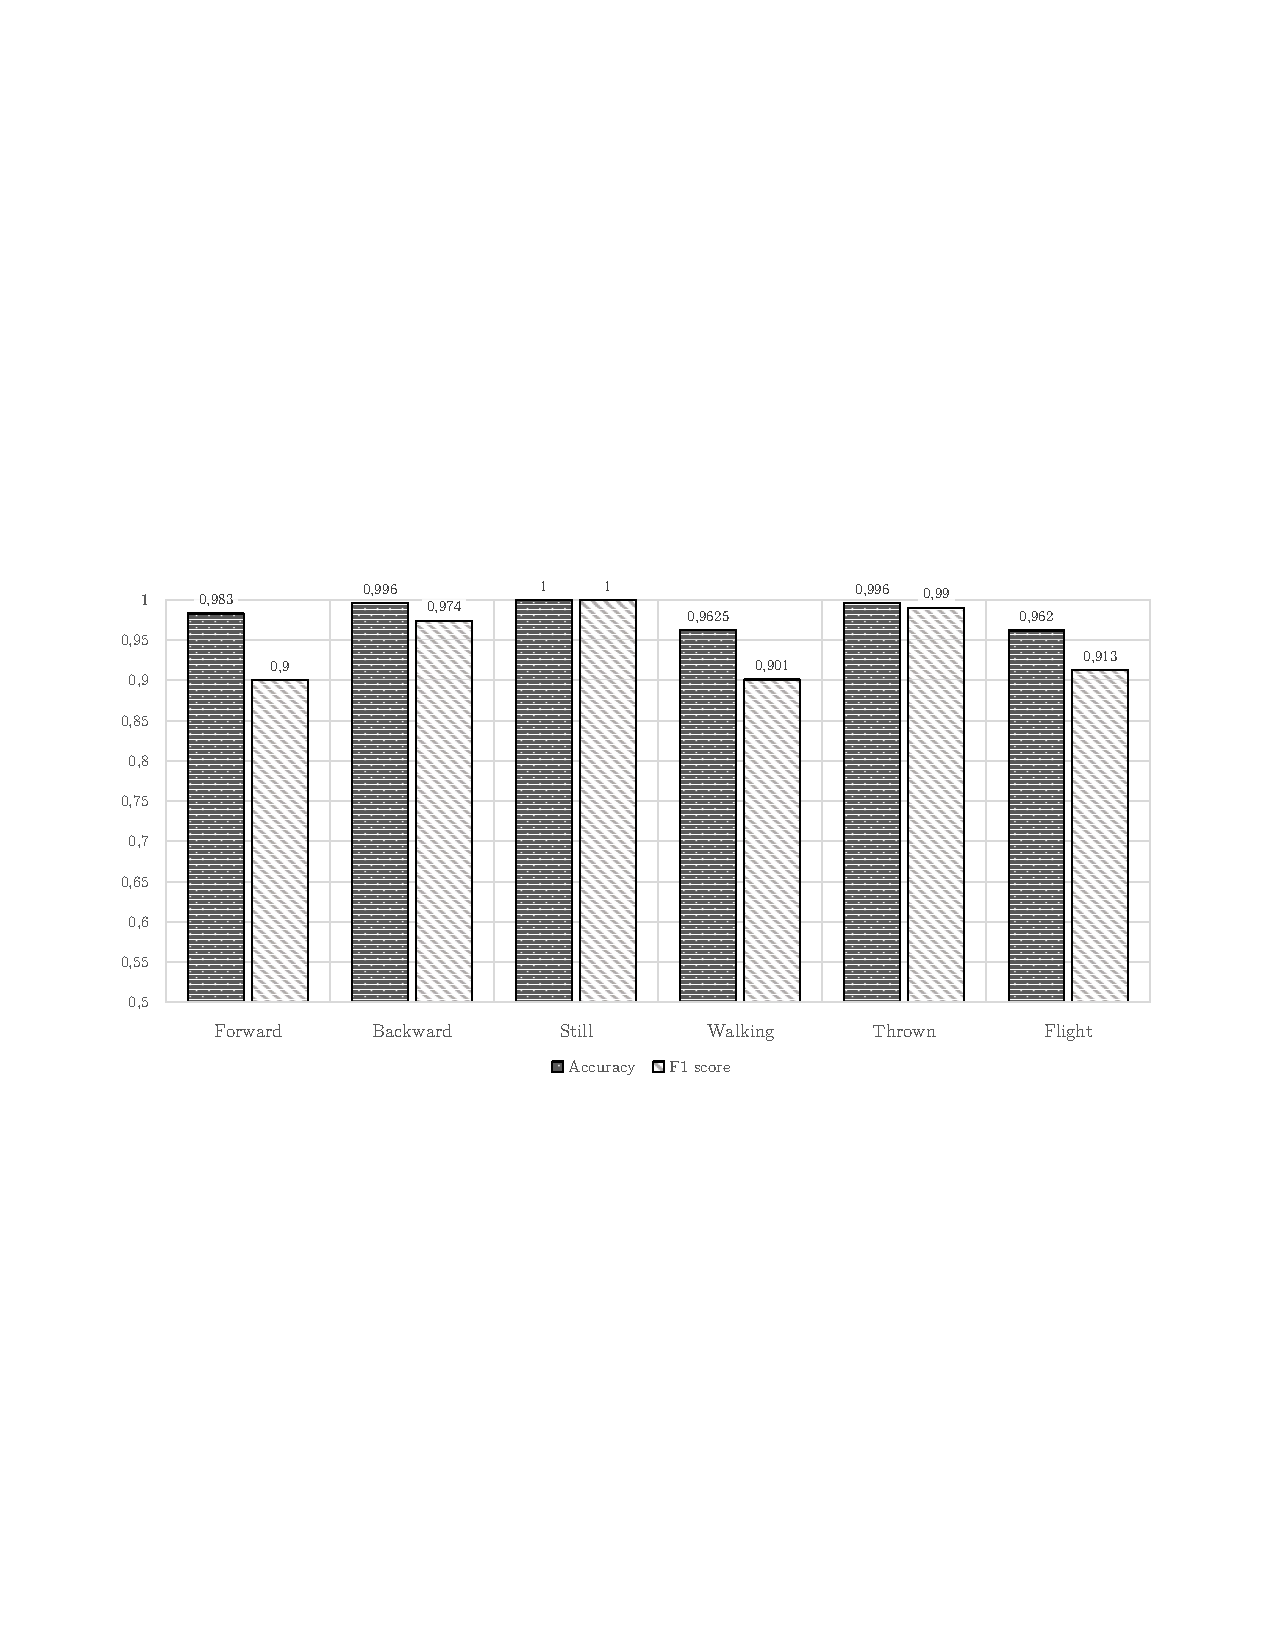
\includegraphics[width=0.8\paperwidth]{img/rnn_results.pdf}}
		\caption{RNN testing results.}
	\end{figure}
\end{center}

\begin{center}
	\begin{figure}[ht!]
		\makebox[\textwidth]{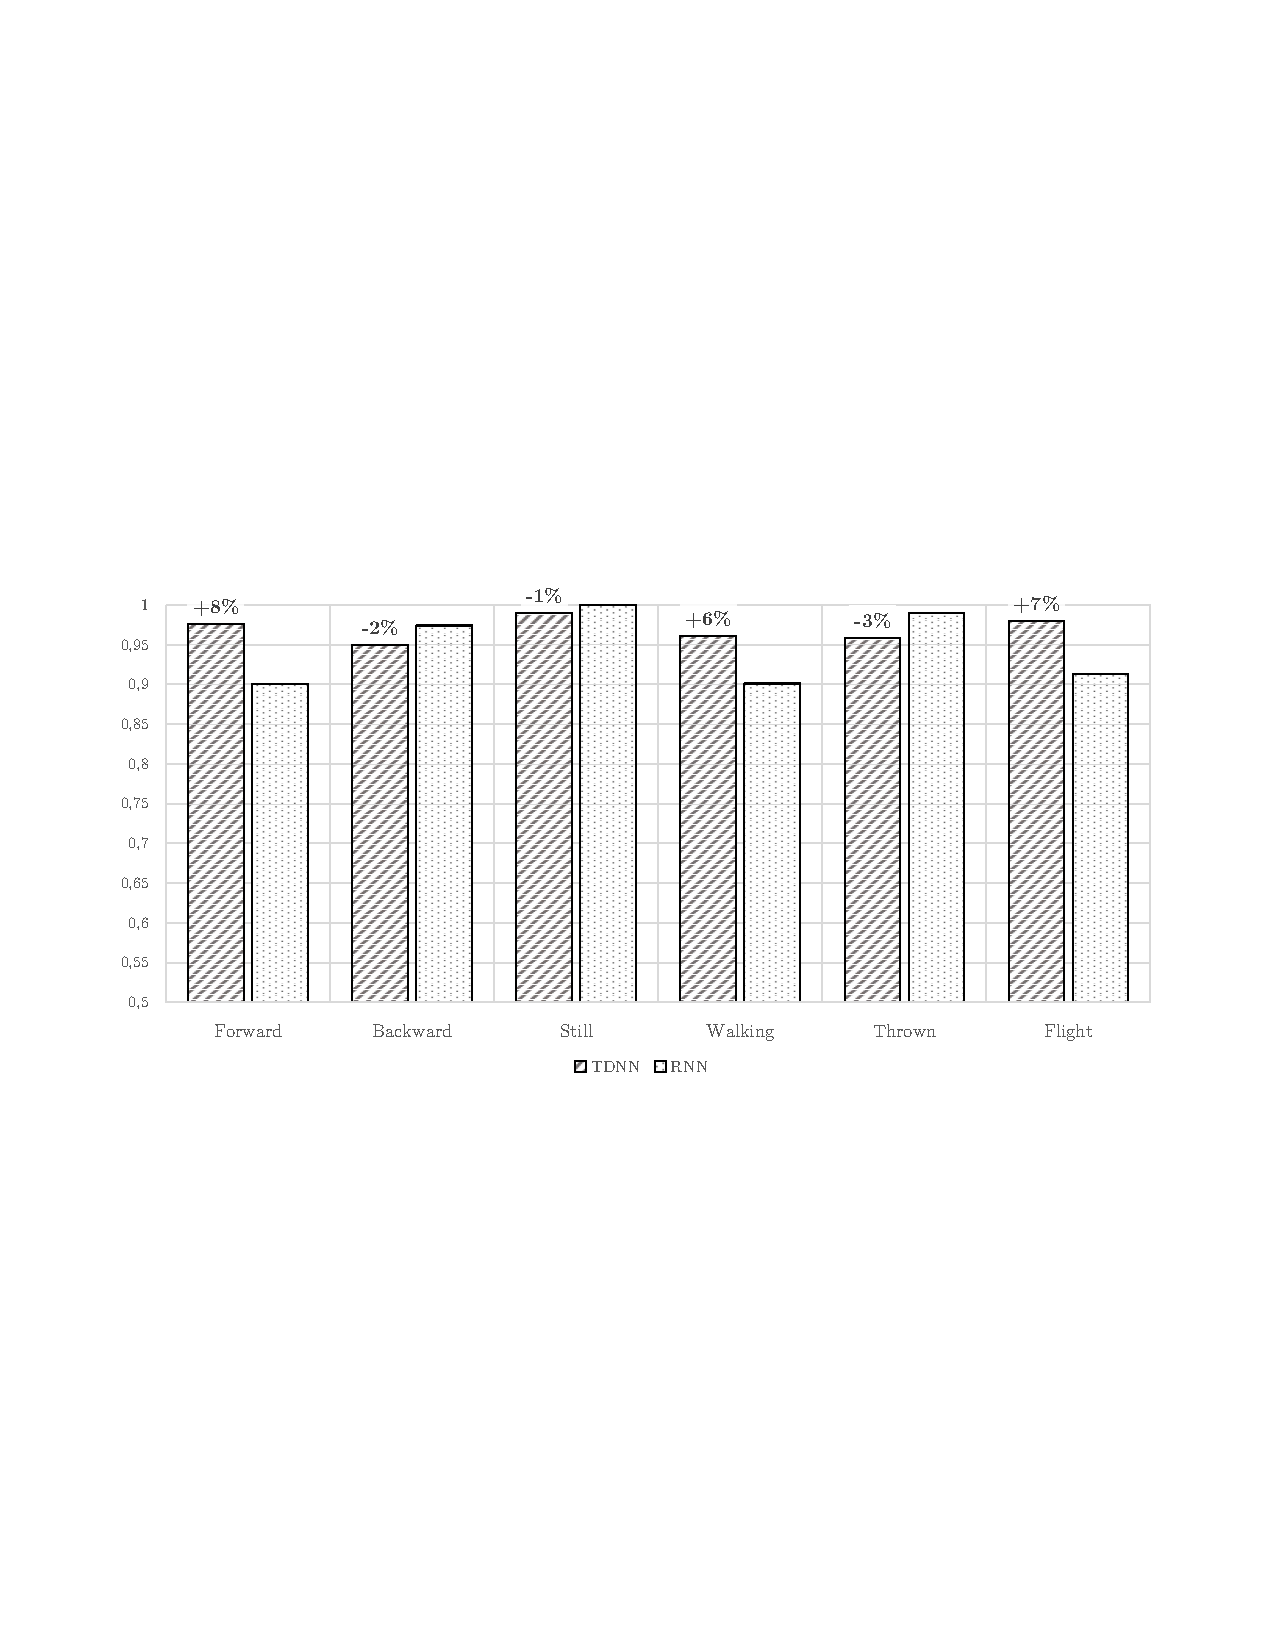
\includegraphics[width=0.8\paperwidth]{img/networks_comparison.pdf}}
		\caption{F1 score comparison between TDNN and RNN.}
	\end{figure}
\end{center}
\clearpage

The high accuracy obtained in validation and testing might not reflect the real network's performances in analyzing real play sessions: in the first two cases, the patterns have a well-defined start and end, while in a play session there is a contiguous stream of data; for the classification, the network is given a fixed-length subsection of that stream for each 22nd of second, and the subsection's bounds slide forward, like a sliding window, through the whole stream. When subsection contains only a single pattern, the networks behaves exactly like in the validation/testing scenario, but when there is an overlapping between two patterns (e.g. the toy stops flying and stays still), the classification is harder, because that's not a case that the network was trained to deal with.
\bigbreak

The following images represents data from a 46 seconds-long session of simulated play, that has been split in four charts for simplicity's sake: the $x$-axis represents the time, the left $y$-axis represents the neural network classification, charted with a black line, and the right $y$-axis represents the intensity of the acceleration among the three dimensions, charted with three different colors. Finally, the colored stripes below the graph represents the ground truth, and the slashes indicates that the classification isn't changing within the omitted period of time. The gray stripe represents the ``still'' condition, but its label has been omitted for better readability.
\bigbreak

The network was able to accurately recognize the \textit{still}, \textit{forward} and \textit{backward} patterns, while in \textit{flight} and especially \textit{walking}, the overall classification is correct, but there are some short misclassifications, visible as spikes in the graph.

\clearpage
\begin{sidewaysfigure}[tbp]
	
\includegraphics[width=\textwidth]{img/plots/session/1.png}
	\vspace{2cm}

	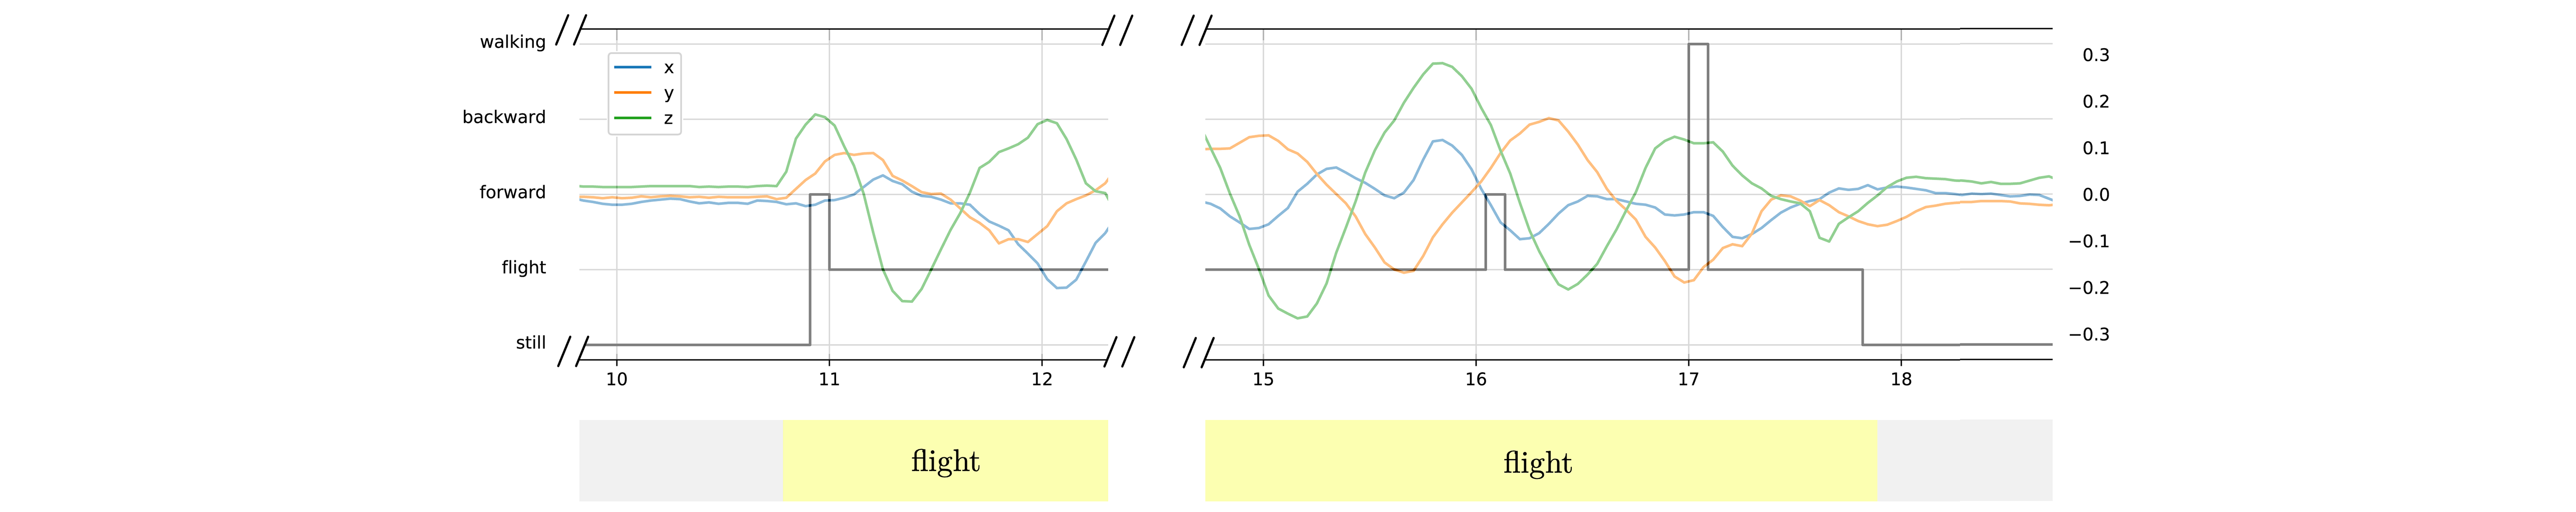
\includegraphics[width=\textwidth]{img/plots/session/2.png}
\end{sidewaysfigure}
\clearpage

\clearpage
\begin{sidewaysfigure}[tbp]
	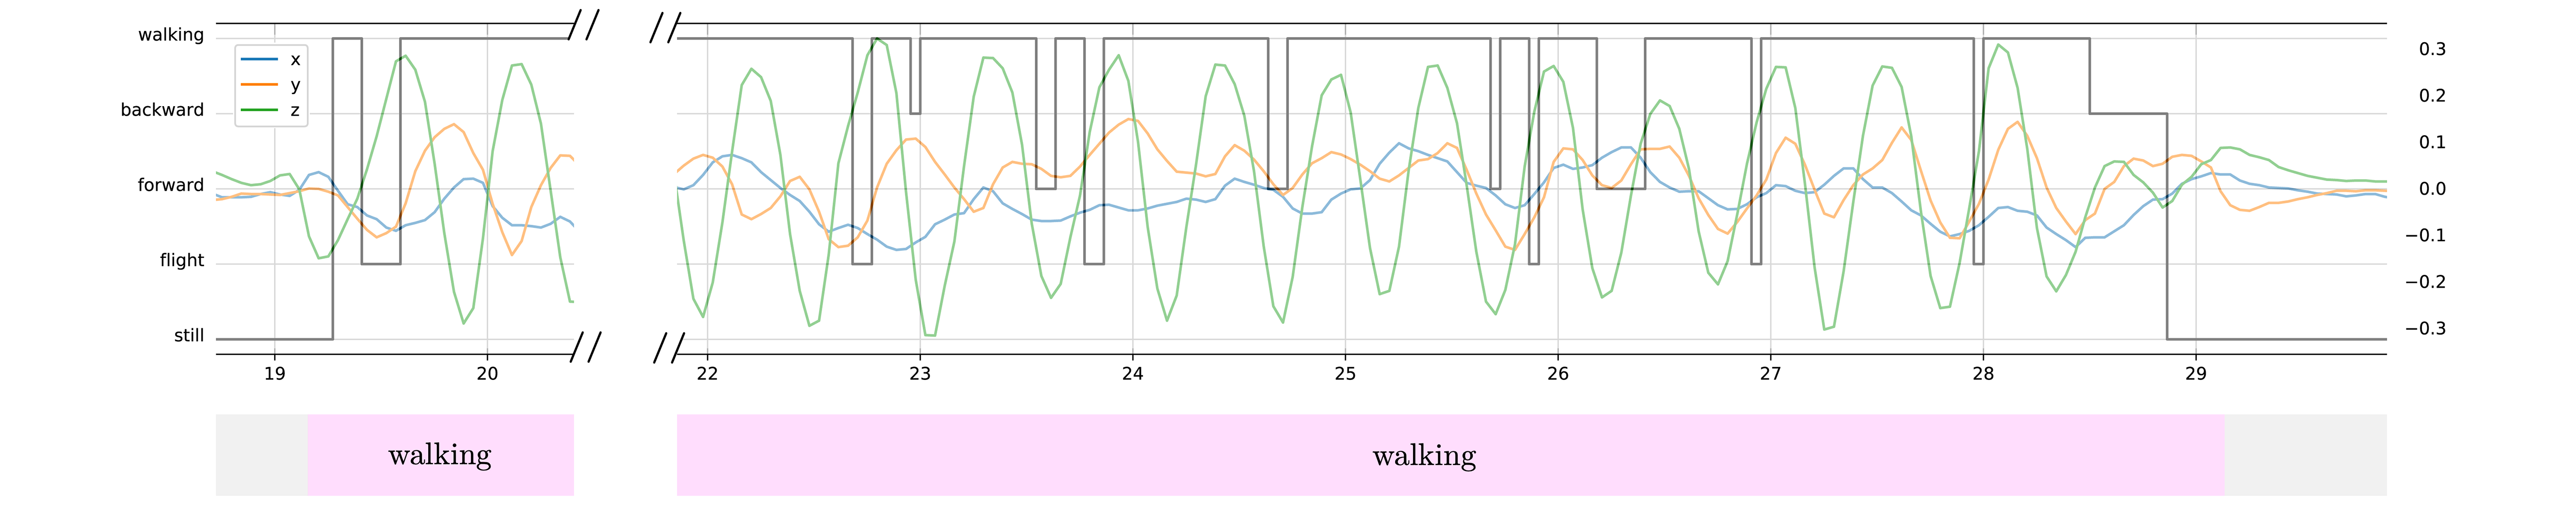
\includegraphics[width=\textwidth]{img/plots/session/3.png}
	\vspace{2cm}

	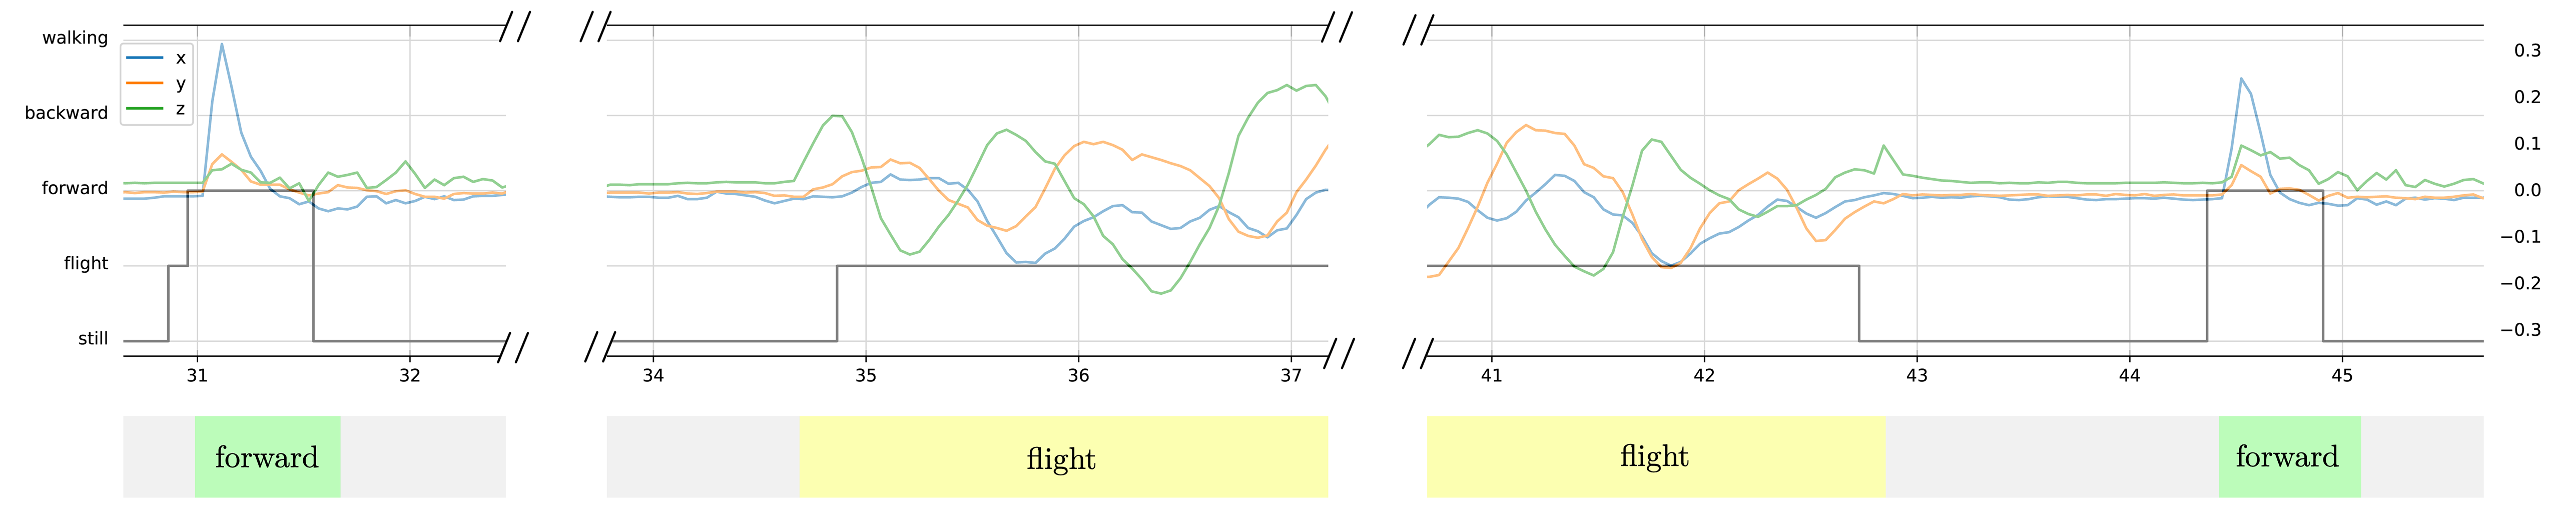
\includegraphics[width=\textwidth]{img/plots/session/4.png}
\end{sidewaysfigure}
\clearpage
